% TODO: Figure out how to call those "programming experiences" (also is this a good name?)
%   the text uses "concrete, collaborative, interactive" - but this is a silly list
%   really, they are "cool" but how to say that.
%
% TODO: Also, what exactly goes into the list?
%
%
\documentclass[sigconf]{acmart}
%\documentclass[sigconf,review,anonymous]{acmart}

\usepackage{hhline,xcolor,colortbl}
\usepackage{fontawesome}
\usepackage{enumitem}
\usepackage{fancyvrb}
\usepackage{tikz}
\usepackage[breakable,theorems,skins]{tcolorbox}
\usepackage{lettrine}

\newcommand{\ident}[1]{{\sffamily #1}}

\newcommand*\circled[1]{\textnormal{\footnotesize\sffamily\bfseries\protect\tikz[baseline=(char.base)]{
  \node[shape=circle,fill=black,text=white,draw,inner sep=1pt] (char) {#1};}}}

\DeclareRobustCommand{\keyideabox}[3]{\begin{tcolorbox}[breakable,
  boxsep=5pt,left=0pt,right=0pt,top=0pt,bottom=0pt,width=\dimexpr\columnwidth\relax,
  colback=gray!20,colframe=gray!20,
  enlarge bottom by=0pt,enlarge top by=0pt,
  arc=0pt,outer arc=0pt]
\lettrine[lraise=0.3]{\LARGE #1}{~}
\small \textbf{#2.} #3
\end{tcolorbox}
}

\setlist{leftmargin=1.5em}
\setlength\itemsep{0.5em}

\setcopyright{acmlicensed}
\copyrightyear{2018}
\acmYear{2018}
\acmDOI{XXXXXXX.XXXXXXX}

\acmConference[Conference acronym 'XX]{Make sure to enter the correct
  conference title from your rights confirmation emai}{June 03--05,
  2018}{Woodstock, NY}
\acmISBN{978-1-4503-XXXX-X/18/06}

\begin{document}
\title[Denicek: Computational Substrate for Concrete, Collaborative, Interactive
  Programming]{{\scshape Denicek}: Computational Substrate for Concrete, \\Collaborative, Interactive Programming}

\author{Tomas Petricek}
\email{tomas@tomasp.net}
\orcid{0000-0002-7242-2208}
\affiliation{%
  \institution{Faculty of Mathematics and Physics, Charles University}
  \city{Prague}
  \country{Czech Republic}
}

\begin{abstract}
Research on interactive programming systems gave rise to a range of programming experiences,
including programming by demonstration, local-first collaborative editing, %structure editing,
schema and code co-evo\-lution, provenance tracking and incremental recomputation. Those
experiences are compelling, but they are hard to implement on the basis of existing programming
languages and systems.

We contribute the Denicek computational substrate. Denicek represents a program as a series of edits
that construct or transform a document consisting of data and formulas. Denicek provides two
primitive operations on series of edits, merging and conflict checking, that form the backbone
of the implementation of the aforementioned programming experiences.

We discuss the architecture of Denicek, document key design considerations and elaborate
the implementation of the programming experiences listed above. To evaluate the proposed
architecture, we use Denicek as the basis of a simple innovative data exploration environment.
The case study shows that the Denicek computational substrate provides a pathway to the design
of richer and more accessible interactive programming systems.
\end{abstract}

\keywords{Do, Not, Us, This, Code, Put, the, Correct, Terms, for,
  Your, Paper}

%\begin{teaserfigure}
%  \includegraphics[width=\textwidth]{sampleteaser}
%  \caption{Seattle Mariners at Spring Training, 2010.}
%  \Description{Enjoying the baseball game from the third-base
%  seats. Ichiro Suzuki preparing to bat.}
%  \label{fig:teaser}
%\end{teaserfigure}
\maketitle

\newpage

\section{Introduction}

Medium is the message

~

~

Lorem ipsum dolor sit amet, consectetur adipisicing elit, sed do eiusmod tempor incididunt ut labore et dolore magna aliqua. Ut enim ad minim veniam, quis nostrud exercitation ullamco laboris nisi ut aliquip ex ea commodo consequat. Duis aute irure dolor in reprehenderit in voluptate velit esse cillum dolore eu fugiat nulla pariatur. Excepteur sint occaecat cupidatat non proident, sunt in culpa qui officia deserunt mollit anim id est laborum.

TODO: Maybe do not talk about ``programs'' because this is more documents with formulas - not that fancy programs.
Computational documents?

explain computational substrate

JUSTIFICATION - this is a technical paper but belongs here!

DESIGN PROCESS = formative examples + evaluation case study


\subsection{Programming Experiences}
list

\subsection{Substrate}
how it works very roughly

The coolest trick - almost everything (PBD, collaboration, evaluation) is done through merge!

\subsection{Contributions}
one main thing - substrate - with other things


\section{Background}
all the references

% ==================================================================================================


\begin{figure*}[t]
\vspace{-0.5em}
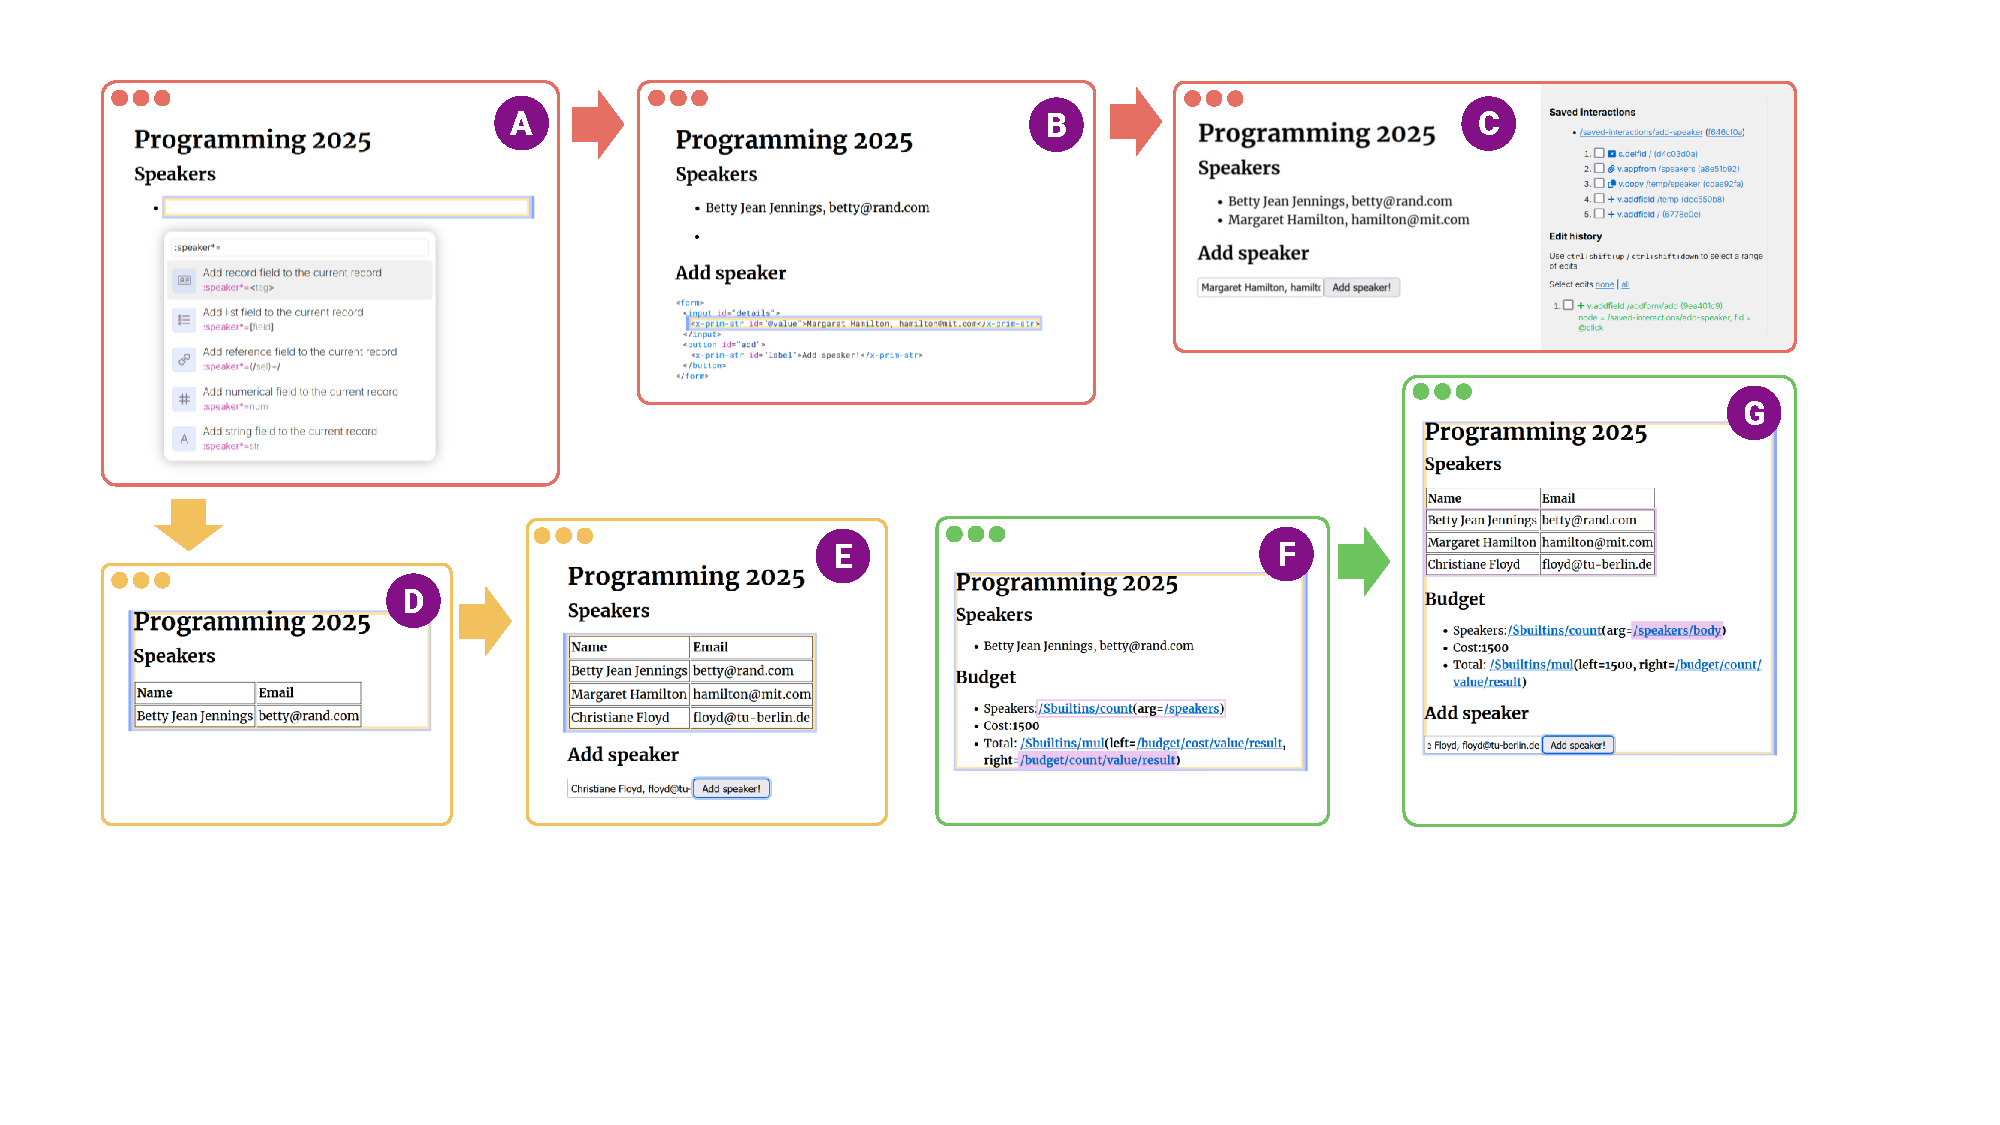
\includegraphics[width=0.95\textwidth,clip,trim=1cm 1cm 1cm 0.5cm]{fig/walkthrough.pdf}
\vspace{-1em}
\caption{Organizing a conference using Denicek. The Walkthrough shows construction of a user
  interface for adding speakers (A, B, C); refactoring of the list and merging edits (D, E); and
  formulas with schema and code co-evolution (F, G).}
\label{fig:walkthrough}
\end{figure*}

\newpage


\section{Walkthrough}
\label{sec:walk}

To providea an overview of the programming experiences supported by the Denicek
substrate, we use a web-based implementation of Denicek with a structure
editor that supports navigation in document and issuing of edit commands. The editor
implements support for a range of programming experiences, discussed in \S\ref{sec:impl}.

\subsubsection*{\circled{A} Adding a Speaker}
The user starts with an empty document, which is represented as a record. They add a field for
each heading and a list {\small\Verb_<ul>_} as a field named {\small\Verb_speakers_}. They use the command
toolbox to add the first speaker.

\subsubsection*{\circled{B} Creating a User Interface} To simplify adding of
further speakers, the user creates a textbox and a button. They enter new speaker
details, construct a temporary {\small\Verb_<li>_} element outside of the main list, copy the value
from the textbox into the new element using source view, and then copy the new element into the
{\small\Verb_speakers_} list.

\subsubsection*{\circled{C} Saving the Interaction} After adding the speaker from the textbox,
the user opens history view, selects edits that added the speaker and saves those as the
{\small\Verb_add-speaker_} interaction. They attach this as a handler for the {\small\Verb_click_} event of the button.

\keyideabox{\faLightbulbO}{Programming by Demonstration}{Denicek implements programming by
demonstration (\S\ref{sec:impl-pbd}) by letting the user to save and replay past interactions,
either directly or by attaching them to a UI event.}

\subsubsection*{\circled{D} Refactoring Document Structure} Another user starts with the initial
version of the document and turns the list into a table. This is done by invoking a series of
commands that change tags, wrap elements, copy and transform values.

\subsubsection*{\circled{E} Merging Edits} The two document versions can be automatically merged.
The refactoring is applied to all existing speakers. New speakers added using the ``Add speaker!''
button are also automatically turned into the new format.

\keyideabox{\faLightbulbO}{Collaborative Editing and Interactivity}{Denicek's merging
reapplies edits from another branch on top of the current history (\S\ref{sec:impl-collab}).
Merging is asymmetic, but the order does not matter here. The same merging operation is used
when handling user interaction (\S\ref{sec:impl-interaction}).}

\subsubsection*{\circled{F} Adding Budget Calculation} A third user adds budget calculation to
the initial document. Formulas are represented as special {\small\Verb_x-formula_} nodes whose arguments
are other nodes or references to other nodes or formulas (highlighted on mouse hover).

\keyideabox{\faLightbulbO}{Incremental Recomputation}{Evaluating a formula yields additional
edits that augment the document with the result. Those edits are kept
at the top of the document history and are removed in case of a conflict (\S\ref{sec:impl-incremental}),
providing incremental recomputation.}

\subsubsection*{\circled{G} Merging Formulas} When the budget calculation is merged with the
other edits, references in formulas are automatically updated to point to the new list.
Adding new speaker via the ``Add speaker!'' button invalidates the evaluated result.

\keyideabox{\faLightbulbO}{Schema Code Co-Evolution}{References are understood
by the substrate and so they are updated by structural edits (\S\ref{sec:impl-schema}). The
evaluation mechanism can replace formulas with values, but also augment them to keep an evaluation
trace for provenance analysis (\S\ref{sec:impl-provenance}).}

% ==================================================================================================

\arrayrulecolor{lightgray}
\definecolor{ekgray}{gray}{0.90}

\begin{figure}
\newcommand{\seltablecol}[3]{
\sffamily\small{\bfseries #2} & {\footnotesize #1} & \footnotesize #3\\
}
\newcommand{\ndtablecol}[4]{
\raisebox{-0.2em}{#1} & \sffamily\small{\bfseries #2}\,\;\textit{\footnotesize #3}\\[-0.2em]
&\sffamily\footnotesize #4\\[0.3em]
}

\begin{tabular}{|llp{18.08em}|}
\hline
\rowcolor{ekgray}
&&\\[-1em]
\rowcolor{ekgray}
\sffamily\small{\bfseries Selector} & {\sffamily\footnotesize Notation} & \\[0.2em]
\hline
&&\\[-1em]
\seltablecol{\Verb|field|}{Field}{Refers to record field of a given name}
\seltablecol{\Verb|number|}{Index}{Refers to list element at a given index}
\seltablecol{\Verb|*|}{Any}{Refers to all children of a list node}
\hline
\end{tabular}

~\\[0.5em]

\begin{tabular}{|cl|}
\hline
\rowcolor{ekgray}
&\\[-1em]
\rowcolor{ekgray}
& \sffamily\small{\bfseries Kind}\;\,\textit{\footnotesize arguments} \\[0.2em]
\hline
&\\[-1em]
\ndtablecol{\faListUl}{List}{tag, child$_1$, $\ldots$, child$_n$}
  {Ordered list of nodes, addressable by index. Renders as \Verb|<tag>| with children}
\ndtablecol{\faFileO}{Record}{tag, field$_1$, child$_1$, $\ldots$, field$_n$, child$_n$}
  {Record with children addressable by \textit{field} name. Renders as \Verb|<tag>|.}
\ndtablecol{\faExternalLink}{Reference}{selectors}
  {Reference to another document location. Displays the \Verb|/selectors| as a link.}
\ndtablecol{\faFont}{Primitivie}{string \textnormal{or} number}
  {Numerical or textual primitive value. Renders as an HTML text node.}
\hline
\end{tabular}
\vspace{-0.5em}
\caption{Structure of selectors and document nodes}
\label{fig:doc}
\vspace{-1em}
\end{figure}

% ==================================================================================================

\section{The Denicek Substrate}
\label{sec:system}
Denicek represents programs as sequences of edits that construct and transform a computational
document. In this section, we describe the structure of documents and edits, as well as the
operations that form the backbone of the system and are used to implement a wide range of
programming experiences, discussed in \S\ref{sec:impl}.

\subsection{Selectors, Documents and Edits}
A computational document is a tree, consisting of four kinds of nodes (Fig.~\ref{fig:doc}).
Denicek follows the \emph{naive realism}~\cite{disessa-1986-boxer} principle and makes the entire
document visible to the user, although parts can be collapsible or hidden using CSS.
Records and lists are rendered as HTML elements of a specified tag with children becoming child
elements. Field names are hidden in the rendered document.

References to document location are used in both document itself (reference nodes) and in edits
(target of the edit). They are represented as a sequence of selectors (Fig.~\ref{fig:doc}).
The document model assumes that lists are homogeneous and records heterogeneous, and so the
\ident{Any} selector makes it possible to refer to all children of a list, but there is no
way to refer to all children of a record.

\subsubsection*{Document Edits}
The supported document edits and their behavior are listed in Fig.~\ref{fig:edits}. All edits
require \emph{target} to which they are applied. Target is a reference and can contain the
\ident{Any} selector, in which case the edit is applied to multiple nodes simultaneously.
Most edits can only be applied to target node(s) of a particular kind.

The edits are designed to allow any transformation of a document
through a series of steps whose effect can be tracked by the substrate. As illustrated earlier,
Denicek updates references when document structure changes. Fig.~\ref{fig:edits} distinguishes
between edits that keep existing references in a document unchanged (above) and edits that affect
references (below). When a selector is \emph{invalidated}, e.g., when deleting a field or a
list item to which there is a reference, Denicek rejects the edit. Copying also invalidates
selectors because it is ambiguous whether selectors referring to the original location should
refer to the source or the target of the copying after the edit (and references cannot refer to
multiple structurally incompatible locations). Updating a field, wrapping, reordering or deleting
a list item requires updating references in the document correspondingly.

% ==================================================================================================

\begin{figure}
\newcommand{\ektablecol}[6]{
\raisebox{-0.2em}{#1} & \sffamily\small{\bfseries #2}\,\;\textit{\footnotesize target, #3} & \sffamily\footnotesize #4 & \sffamily\footnotesize #5 \\[-0.2em]
&\multicolumn{3}{l|}{\sffamily\footnotesize #6}\\[0.3em]
}
\begin{tabular}{|cp{13em}rr|}
\hline
\rowcolor{ekgray}
&&&\\[-1em]
\rowcolor{ekgray}
 & \sffamily\small{\bfseries Edit}\;\,\textit{\footnotesize arguments} & \sffamily\footnotesize\bfseries Target & \sffamily\footnotesize\bfseries Selectors \\[0.2em]
\hline
&&&\\[-1em]
\ektablecol{\faPlus}{Add}{field, node}{Record}{Unchanged}
  {Add \textit{node} as a \textit{field} to the specified record.}
\ektablecol{\faAt}{Append}{node}{List}{Unchanged}
  {Append \textit{node} to the end of the specified list.}
\ektablecol{\faPaperclip}{AppendFrom}{selectors}{List}{Unchanged}
  {Append node from \emph{selectors} to the end of the specified list.}
\ektablecol{\faICursor}{PrimitiveEdit}{transform}{Primitive}{Unchanged}
  {Apply primitive \textit{transform} to the specified primitive.}
\ektablecol{\faCode}{UpdateTag}{old tag, new tag}{Tagged}{Unchanged}
  {Change the tag of a specified list or record from \textit{old} to \textit{new}.}
\hline
&&&\\[-1em]
\ektablecol{\faFont}{UpdateField}{old field, new field}{Record}{Update}
  {Rename the field of a specified record from \textit{old} to \textit{new}.}
\ektablecol{\faTimesCircle}{DeleteField}{field}{Record}{Invalidate}
  {Delete the field \textit{field} of a specified record.}
\ektablecol{\faMinusCircle}{DeleteItem}{index}{List}{Update}
  {Delete the item at a given \textit{index} of a specified list.}
\ektablecol{\faSort}{Reorder}{permutation}{List}{Update}
  {Reorder items of a specified list according to a \textit{permutation}.}
\ektablecol{\faFileO}{WrapRecord}{tag, field}{Any}{Update}
  {Wrap the specified node as a \textit{field} of a new record with \textit{tag}.}
\ektablecol{\faListUl}{WrapList}{tag}{Any}{Update}
  {Wrap the specified node as a sole element of a new list with \textit{tag}.}
\ektablecol{\faCopy}{Copy}{selectors}{Any}{Invalidate}
  {Copy nodes(s) from \textit{selectors}, replacing the specified target(s). }
\hline
\end{tabular}
\vspace{-0.5em}
\caption{Summary of document edit types in Denicek}
\label{fig:edits}
\vspace{-1em}
\end{figure}

% ==================================================================================================

\subsubsection*{Automatic Reference Update}
There are two situations in which automatic update of references is undesirable. If an edit is
applied to a singular element of a list (reference contains the \ident{Index} selector),
references that refer into any element of the list should be unchanged.  Such edits may turn
document into an inconsistent state, but they typically do so temporarily during document
construction (checking such edits is discussed in \S\ref{sec:discuss-future}).

Documents can also contain values that can be of multiple different kinds (i.e., a union type).
In such case, references should not be updated when the kind of the value changes. For example,
a formula may be either unevaluated or evaluated. As discussed in \S\ref{sec:impl-eval}, evaluation
involves wrapping, but this should not affect references to the formula.
To support those cases, it is possible to annotate edits that normally affect selectors
(Fig.~\ref{fig:edits}, below) as non-structural. This annotation is required when the
target reference contains the \emph{Index} selector.

\subsubsection*{No Conditional Edits.}
An important aspect of the design is that the effect an edit has on references inside
the document does not depend on the current value of the document. This makes it possible to
define merging solely in terms of edits, without reference to current document state.
(The effect of \ident{Copy} depends only on the existing document structure, but not on its value;
while \ident{AppendFrom} affects only single list element and is thus labelled as a
non-structural edit.)

This design choice makes it impossible to encode computational logic directly in the edits
(e.g., through conditional edits). As we will see in \S\ref{sec:impl-interaction}, such logic
has to be provided as an additional  mechanism on top of the underlying Denicek substrate.

\subsection{Primitive Operations}
\label{sec:system-ops}
Denicek provides three primitive operations. A sequence of edits can be applied to a document, two
sequences of edits can be checked for conflicts or merged. Denicek identifies edit histories by
a (git-like) hash, computed from the hash of the parent and the current edit, which is used to identify
common shared part of the history during conflict checking and merging.

\subsubsection*{Applying Edits}
When applying an edit, Denicek locates the target node and transform it according to the
edit. If the edit may affect references in the document (Fig~\ref{fig:edits}, below), Denicek
updates matching references in the document according to the rules shown in Fig.~\ref{fig:updates}
provided that (i) the edit is not explicitly marked as non-structural, and (ii) the target
reference does not contain \ident{Index} selector, i.e., it targets all elements of any involved
lists. Also note that matching references in the document may be more specific than the edit
target. For example, if we rename {\small\Verb|old|} to {\small\Verb|new|} at {\small\Verb|/foo/*|},
a reference {\small\Verb|/foo/3/old|} will become {\small\Verb|/foo/3/new|}. If the document
contains a reference that would be invalidated by an edit, the edit is rejected.

\subsubsection*{Conflict Detection}
Two edits are conflicting if the order in which they are applied matters. This is the case if
they target the same node, or if one targets a node that is nested inside the node targetted by
the other. For edits with dependencies (\ident{AppendFrom} and \ident{Copy}), a conflict also
occurs if the other edit modifies the dependency.

Given two edit histories, one way to resolve conflicts is by removing (or marking as disabled) all
edits from one of the histories that conflict with edits done by the other history. To do this,
we first collect all targets of edits in the other history. We then iterate over edits from the first
history to see if they depend on or target any of the affected targets. If an edit is removed,
its target reference is added to the set of affected targets, so that other subsequent edits that depend
on its original result are also removed.

\subsubsection*{Merging Edit Histories}
Removing all conflicting edits is sometimes useful, but there are many cases where conflicting
edits, in the above sense, can be reconcilliated. Say we have edit histories with
the same common shared part $E, E_1$ and $E, E_2$. If the edits in $E_1$ and $E_2$ conflict,
the results of applying $E, E_1, E_2$ and $E, E_2, E_1$ would be different. We can, however,
construct edit histories $E_1'$ and $E_2'$ such that the results of applying $E, E_1, E_2'$ and
$E, E_2, E_1'$ are the same.

The key operation that enables such reconcilliation takes two individual edits that occurred
indpendently, $e_1$ and $e_2$, and produces $e_1'$ that has the same logical effect as
$e_1$, but can be applied after $e_2$. There are two aspects of such reconcilliation:

\begin{enumerate}
\item \emph{Apply Edit to Newly Added.} If $e_1$ is adding a new list item, but~$e_2$ is
  changing elements of the target list, we apply the edit $e_2$ to the node added by $e_1$ so
  that, when it is added after the transformation, the added node has the new structure.

\item \emph{Transform Matching References.} If $e_1$ targets a node that is inside a node
  whose structure is changed by $e_2$, the target reference in $e_1$ is updated in a way that
  corresponds to the new structure. That is, using the same rules, shown in Fig.~\ref{fig:updates},
  that apply when transforming references inside a document.
\end{enumerate}

Applying an edit to a newly added node involves a number of cases. When the new node is added
using \ident{Add} or \ident{Copy}, but the target location is modified, this is an unresolvable
conflict (because those two operations would overwrite existing nodes). When the new node is
added as a new list item using \ident{Append}, it can be transformed (by applying the other
edit direclty to the new node).

Finally, when the new node is added using \ident{AppendFrom},
it is copied from another document location. We cannot transform the node in the soource location
(this would have unintended effects) or after adding it (we do not know its new index because of
aforementioned \emph{non-conditionality} of edits). Denicek reconcilliates such edits by first
copying the source node to a new temporary location, transforming it there and then using
\ident{AppendFrom} from the temporary location.


% ==================================================================================================

\begin{figure}
\newcommand{\tttablecol}[5]{
\small{\bfseries #1}\;\,\footnotesize\textit{#2}\,\; --\,\; #5\\[-0.1em]
\quad \footnotesize #3 \;\;$\Rightarrow$\;\; #4 \\[0.3em]
}
\begin{tabular}{|l|}
\hline
\\[-1em]
\tttablecol{UpdateField}{target, old field, new field}{\Verb|/target/old\_field/nested|}{\Verb|/target/new\_field/nested|}
  {Replace Field for matching references.}
\tttablecol{DeleteItem}{target, index}{\Verb|/target/n/nested|}{\Verb|/target/(n-1)/nested|}
  {Decrement Index greater than $n$ in matching refs.}
\tttablecol{Reorder}{target, permutation}{\Verb|/target/n/nested|}{\Verb|/target/permutation(n)/nested|}
  {Update Index using permutation in matching refs.}
\tttablecol{WrapRecord}{target, tag, field}{\Verb|/target/nested|}{\Verb|/target/field/nested|}
  {Insert extra Field selector after matching prefix.}
\tttablecol{WrapList}{target, tag}{\Verb|/target/nested|}{\Verb|/target/*/nested|}
  {Insert extra All selector after matching prefix.}
\hline
\end{tabular}
\vspace{-0.5em}
\caption{How document edits transform references}
\label{fig:updates}
\vspace{-1em}
\end{figure}

% ==================================================================================================


\section{Programming Experiences Implementation}
\label{sec:impl}

The key claim of this paper is that the computational substrate described in the previous
section makes it easy to support a range of experiences that make programming more concrete,
collaborative and interactive. In this section, we describe how to use the substrate to support
local-first collaborative editing (\S\ref{sec:impl-collab}), programming by
demonstration (\S\ref{sec:impl-pbd} and \S\ref{sec:impl-interaction}),
schema and code co-evolution (\S\ref{sec:impl-schema}), incremental recomputation
(\S\ref{sec:impl-eval} and \S\ref{sec:impl-incremental}), provenance tracking (\S\ref{sec:impl-provenance})
and concrete programming via managed copy \& paste (\S\ref{sec:impl-copy}).
We describe the programming experience in isolation in this section. Next section provides a
more comprehensive evaluation through a case study that combines multiple of them together.


\subsection{Local-First Collaborative Editing}
\label{sec:impl-collab}

The Denicek representation enables \emph{local-first} collaboration~\cite{kleppmann-2019-local},
as illustrated in \S\ref{sec:walk}E. If a document is edited by multiple users, they can
each make edits to their local copy and eventually merge document variants using the operation to
merge edit histories.

Merging of histories behaves akin to git rebase in that it keeps a linear history. Synchronization
in a distributed system thus requires first reapplying local edits on top of the remote history,
before updating the remote history. Denicek thus implements the \emph{convergence model} of
document variants \cite{edwards-2025-schema}, i.e., the user cannot, for example, maintain their
own local document structure and import new data from another variant (this would require an
inverse of the edit reconcilliation operation).

Merging of edit histories is not symmetric. Document $D$ in Fig.~\ref{fig:merging}
can be obtained either by appending $C'$ (produced by the edit reconcilliation operation)
on top of $A,B$ or by appending $B'$ on top of $A,C$. Although the two edits are conflicting,
$C$ only affects data and $B$ only affects structure and so the resulting document is the same
in both cases. However, the histories differ. In the first case, the new node added by the
\ident{Append} edit is transformed (from primitive string to a record representing table row).
In the second case, the structural transformations are automatically applied to all rows.
As discussed in \S\ref{sec:system-ops}, conflicts during merging can be resolved either by
removing conflicting edits or by letting the later edits overwrite the former ones.


\begin{figure}[t]
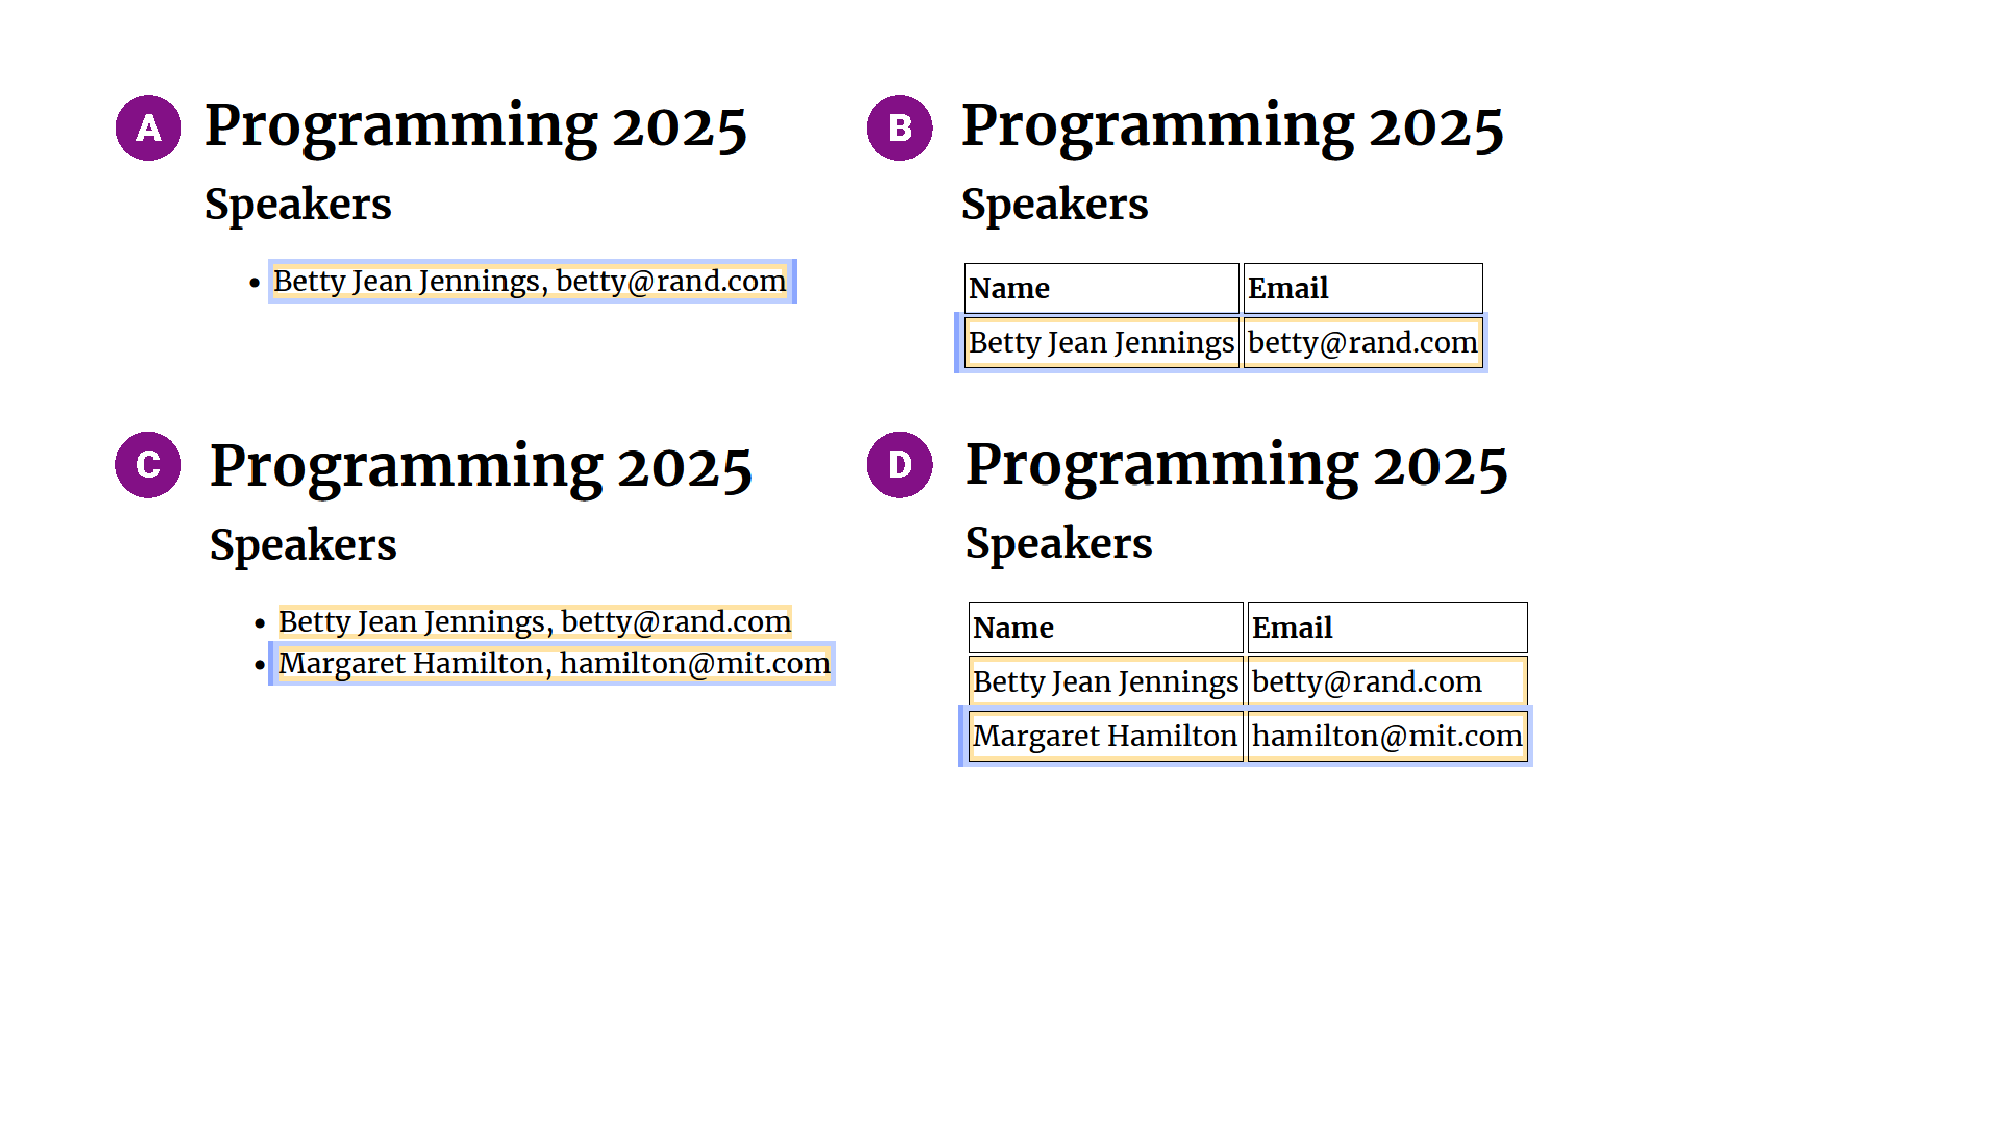
\includegraphics[width=0.9\columnwidth,clip,trim=1.7cm 6cm 7.8cm 1.5cm]{fig/merging.pdf}
\vspace{-0.5em}
\caption{Merging of two independently done sequences of edits. Two ways of merging B and C result in the same D.}
\label{fig:merging}
\vspace{-0.5em}
\end{figure}

\begin{figure}[t]
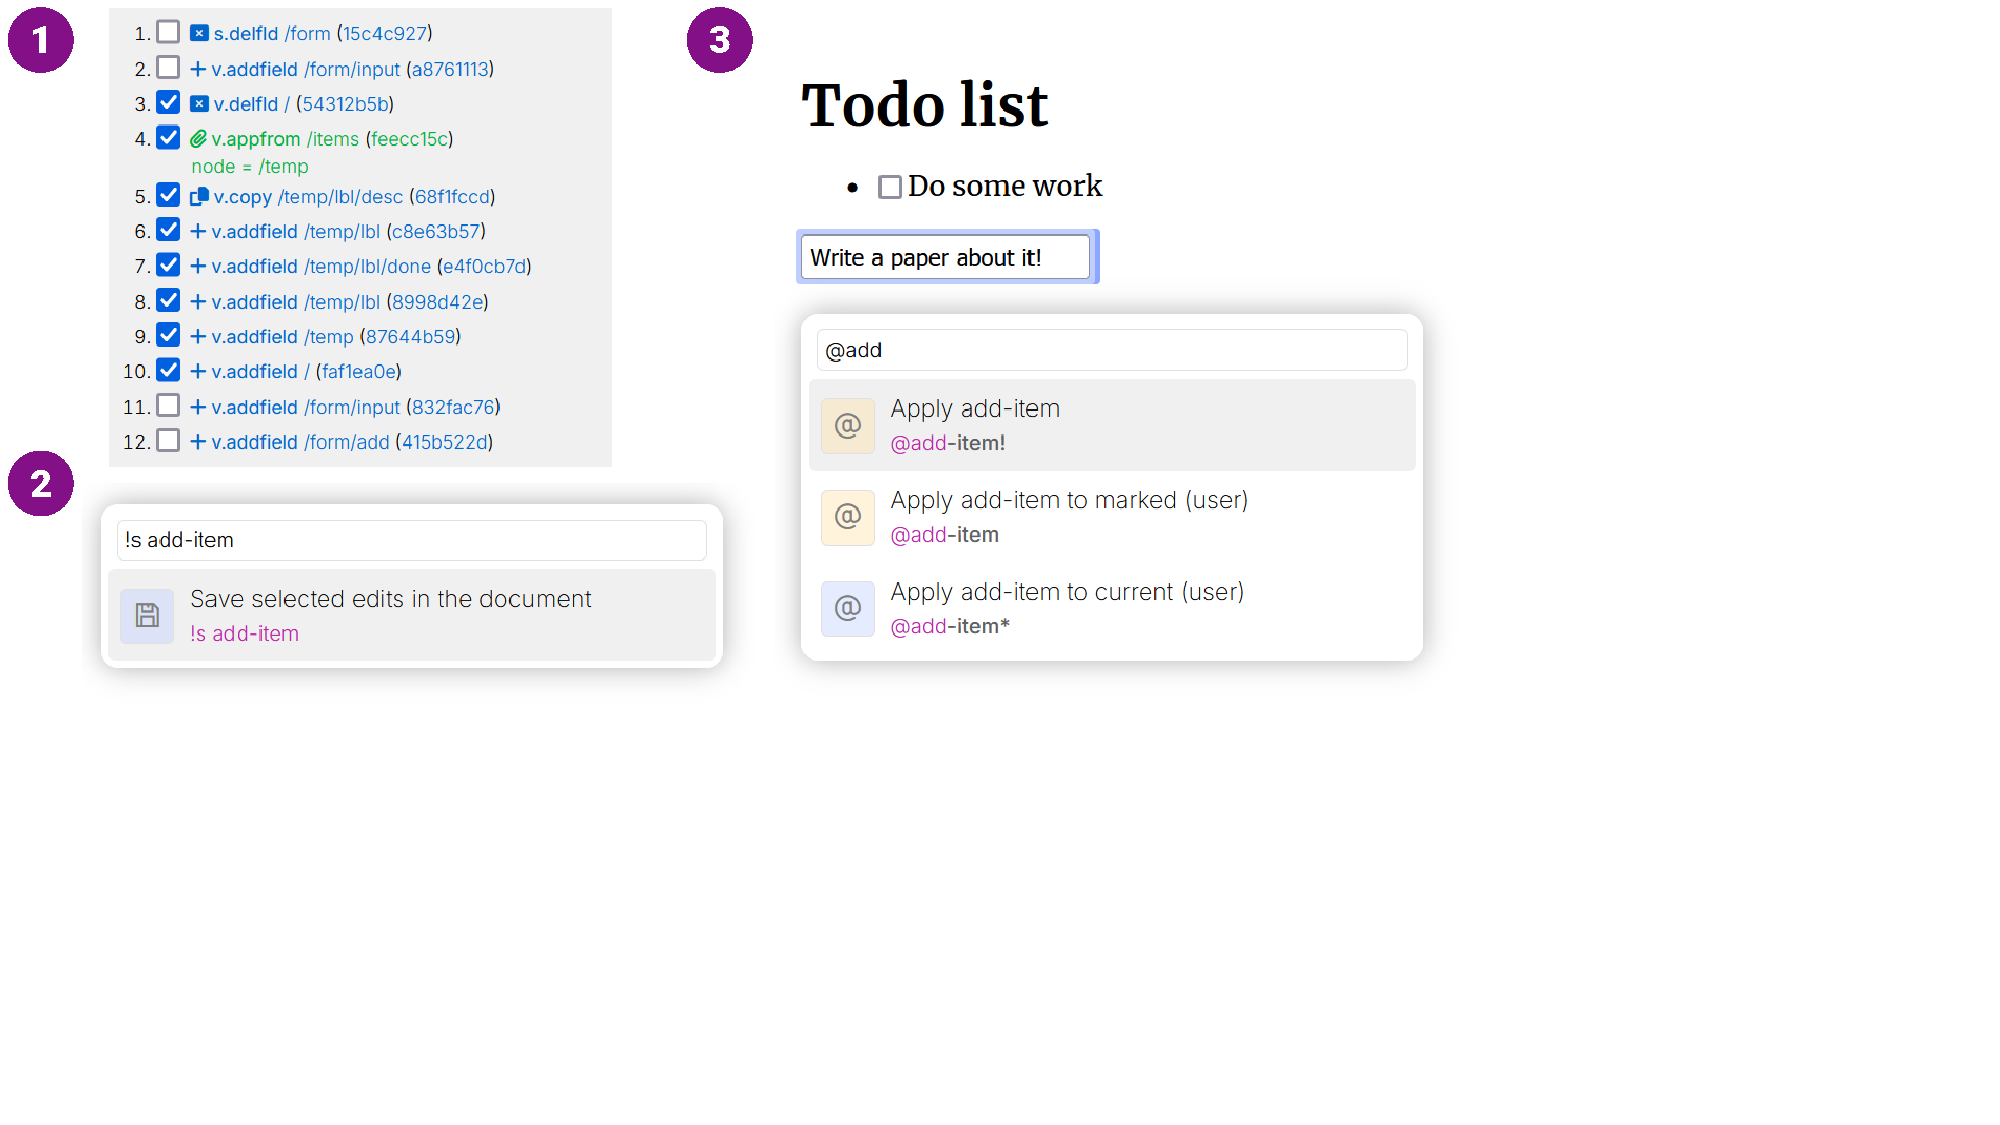
\includegraphics[width=0.9\columnwidth,clip,trim=0cm 7cm 9cm 0cm]{fig/pbd.pdf}
\vspace{-0.5em}
\caption{Programming by demonstration is implemented by selecting edits from the document
history (1), saving them in the document (2) and replaying them (3).}
\label{fig:pbd}
\vspace{-0.5em}
\end{figure}

\subsection{Programming By Demonstration}
\label{sec:impl-pbd}

In \emph{programming by demonstration} \cite{cypher-1993-pbd}, the user demonstrates a task to the
system and the system then repeats it, directly or in a generalized way. To use direct
repetition with Denicek (Fig.~\ref{fig:pbd}), the user can select edits from the edit history,
name them and replay them. In case of general-purpose document editing (in our formative prototype),
this requires certain forethought (e.g., constructing a new list item in a temporary document
field before appending it), but as illustrated in \S\ref{sec:case}, the mechanism is effective in
a restricted domain such as data wrangling \cite{kandel-2011-wrangler}.

There are two notable aspects of our implementation. First, Deni\-cek saves edits in the document
itself (by representing individual edits as nodes and storing them in list inside a
{\small\Verb_<saved-interactions>_} field). This means that no other implementation mechanism
outside of the system is needed and also that the stored edits can be modified by the user
(or tools working with the document).

Second, to replay edits, Denicek does not simply append them on top of the current history.
When saving edits, it records the hash of the history at the time of saving. When replaying edits,
it appends the saved edits to the top of the original history (at the time of saving) and merges this new
sequence with the current history. This pushes the saved edits through all subsequent edits made
by the user. The result can be seen in Fig.~\ref{fig:walkthrough} (E), where a newly added speaker
is transformed from a primitive string to a table row.

The implementation also has to account for the case where edits saved in the document are themselves
transformed (when they are reconcilliated with other edits during merging). In this case, Denicek
updates the saved edits (as discussed in \S\ref{sec:discuss}, this would not be needed if the
history was stored as a graph, akin to ordinary git merging rather than rebasing).

\begin{figure}[t]
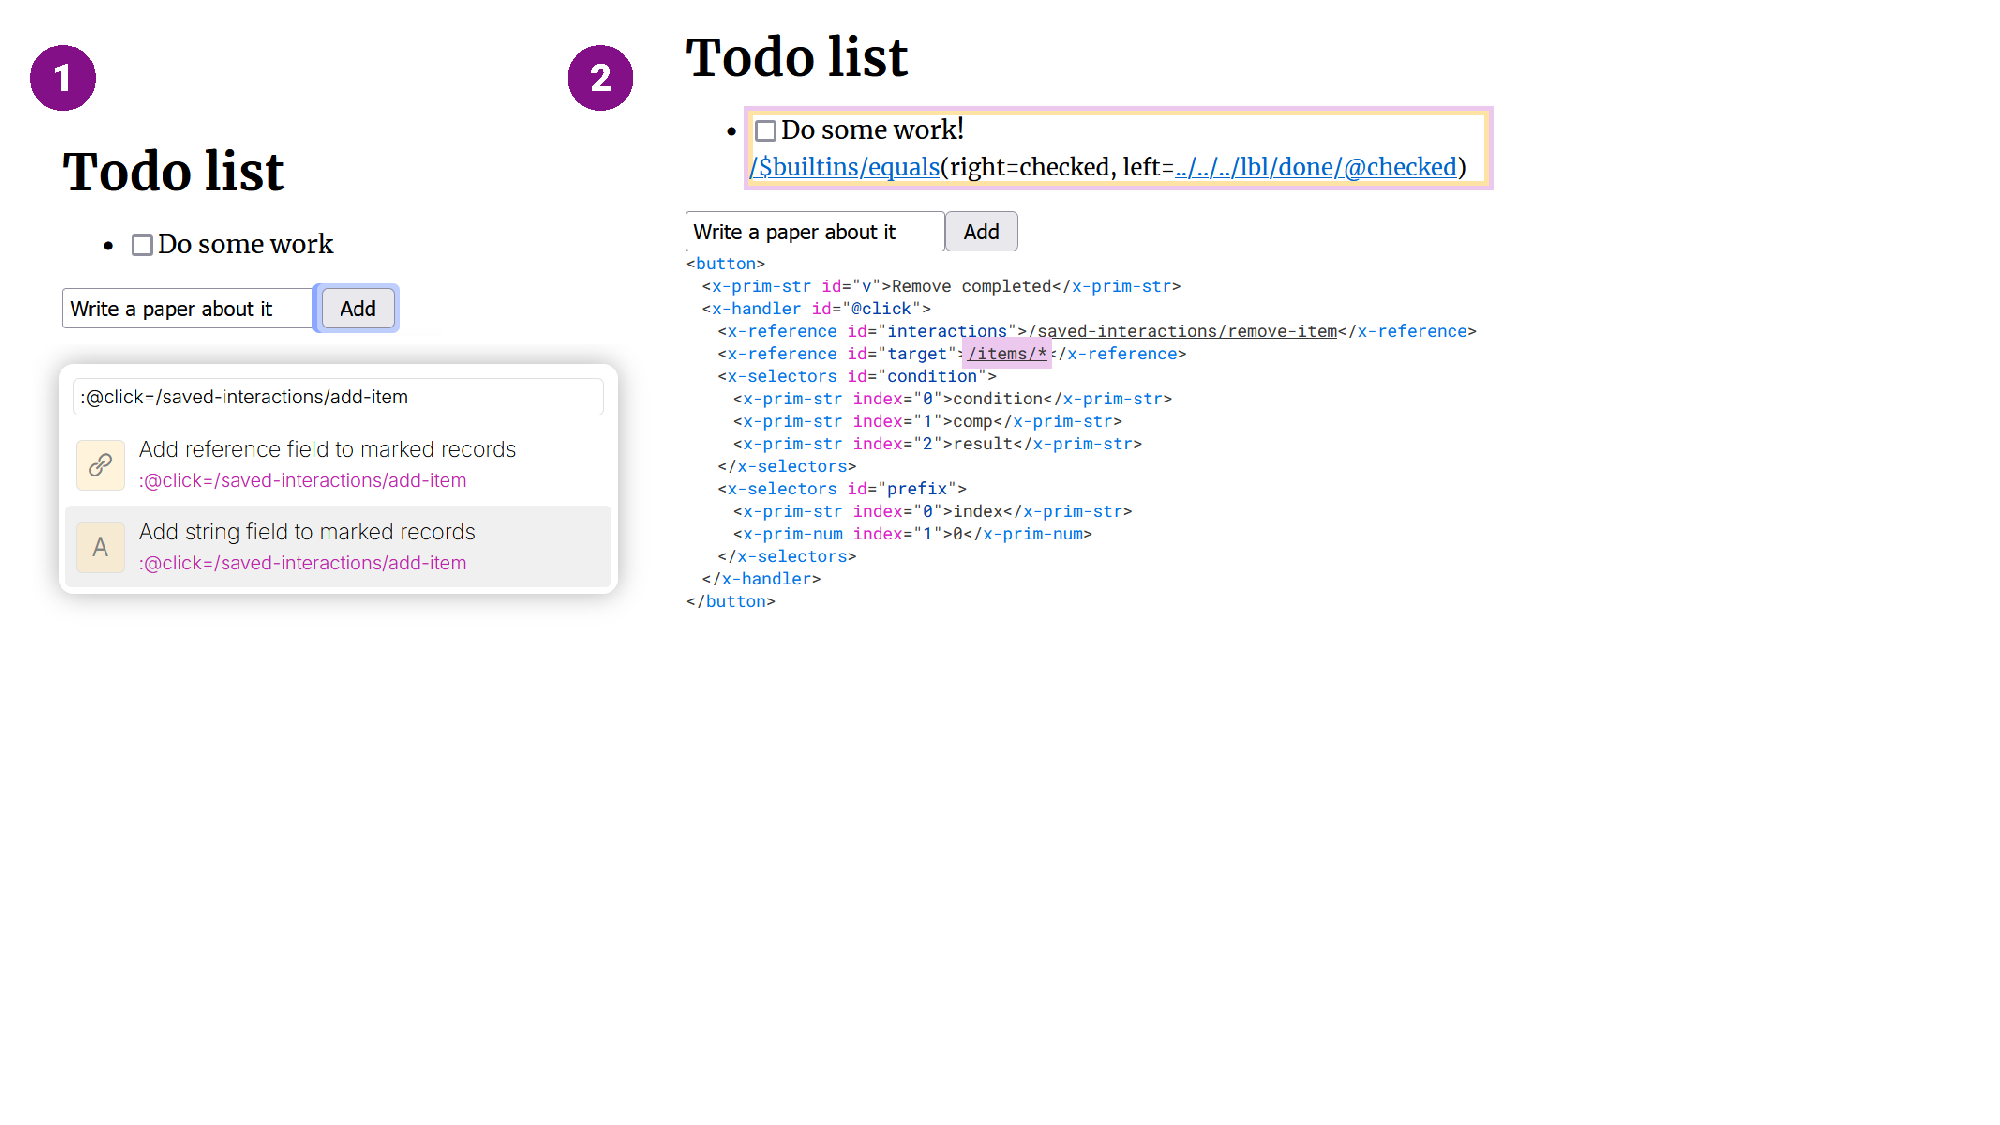
\includegraphics[width=1\columnwidth,clip,trim=0.5cm 8.5cm 8.5cm 0.5cm]{fig/interactive.pdf}
\vspace{-1em}
\caption{Using programming by demonstration to define a UI. The ``Add'' button (1) replays edits;
the ``Remove completed'' button (2) modifies target and specifies a condition. }
\label{fig:interactive}
\vspace{-0.5em}
\end{figure}

\subsection{Interactive User Interfaces}
\label{sec:impl-interaction}

Programming by demonstration can be used to define interactive elements in the document. In the
simple case (Fig.~\ref{fig:interactive} (1)), the {\small\Verb_click_} event handler is set to a
reference to a sequence of edits saved in the document. Clicking the button executes the edits
using the mechanism discussed in \S\ref{sec:impl-pbd}, i.e., by appending them to a history at the
time of saving and merging them with the current history.

The Denicek substrate can be used to generalize the interactions saved through programming by
demonstration. Our prototype illustrates this option in a limited way. As shown in
Fig.~\ref{fig:interactive} (2), a button to remove all completed TODO items can be generalized
from the {\small\Verb_remove-item_} interaction, which removes the list item at the index 0.
In addition to the saved interaction, we manually specify (in the source view) that the edits
should be applied to all elements selected by the {\small\Verb_/items/*_} selector, instead of
the original {\small\Verb_/items/0_} selector (prefix) and that the edits should only be
applied to elements for which the formula (which tests if the checkbox is checked) specified by a
relative selector {\small\Verb_./condition/comp/result_} evaluates to true.

Specifying such generalization manually is cumbersome, but a programming by demonstration system
that implements typical heuristic for generalization from examples \cite{myers-2000-intelligence}
would be able to infer and suggest such generalization to the user (possibly also automatically
adding the formula based on positive and negative examples of selected items).

\begin{figure}[t]
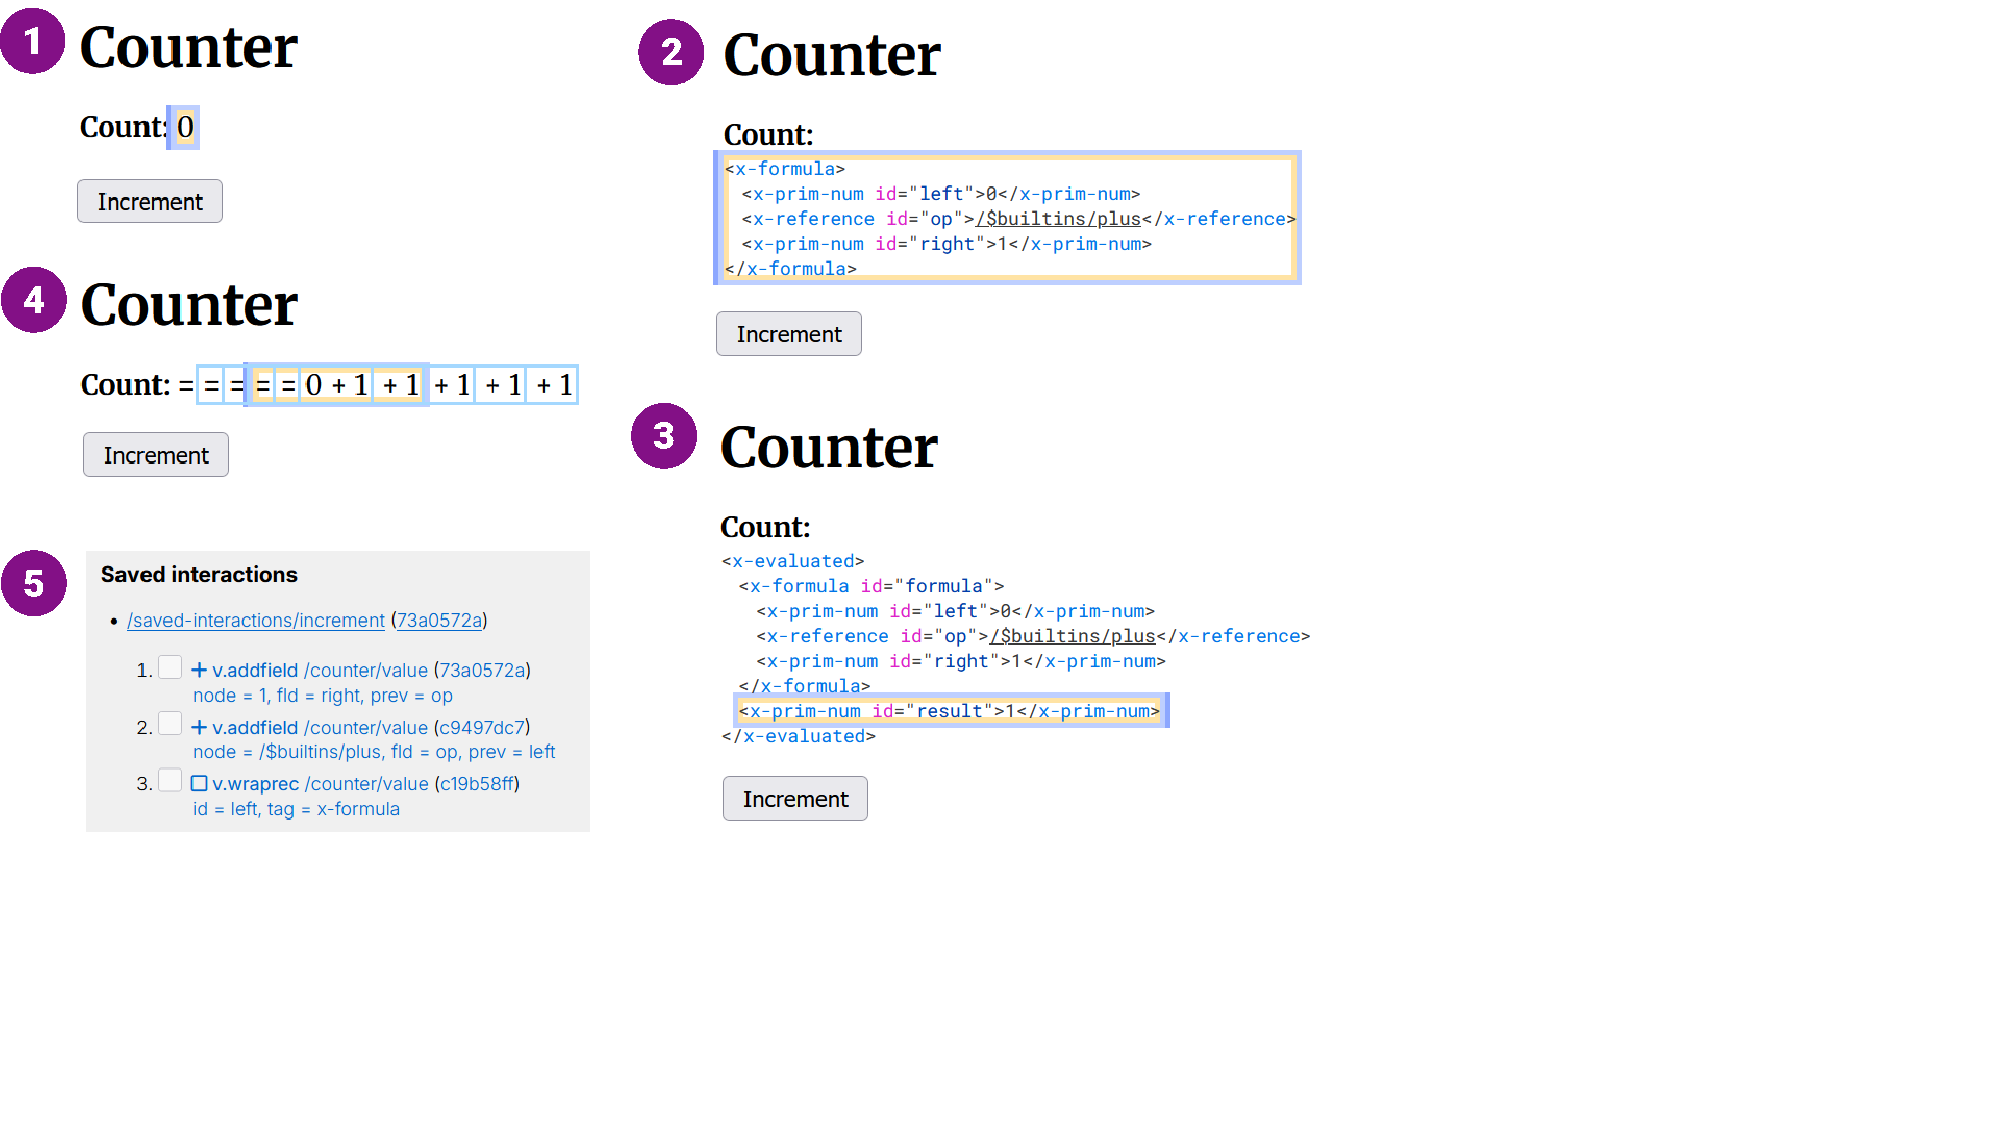
\includegraphics[width=0.95\columnwidth,clip,trim=0cm 7cm 8cm 0cm]{fig/counter.pdf}
\caption{Increment wraps the existing count in a formula that adds 1 to the
previous value (1), (2). Evaluation produces the count (3), which is invalidated on subsequent clicks (4).}
\label{fig:counter}
\vspace{-0.5em}
\end{figure}

\subsection{Formula Language and Evaluation}
\label{sec:impl-eval}

Denicek documents can contain formulas inspired by the spreadsheet
paradigm \cite{nardi-1990-spreadsheets}. Formulas can specify richer computations than
what can be expressed using document edits. Formulas do not transform the document and their
results are transient, although their evaluation also leverages the substrate operations,
namely merging of edit histories.

As illustrated in Fig.~\ref{fig:counter}, formulas are represented as document nodes with a
special tag ({\small\Verb_<x-formula>_}). They are recognized by a formula evaluator and
rendered in a special way (\circled{1} and \circled{4}), but they are created using ordinary
edits and the Denicek substrate treates them as stnadard nodes.

To evalaute formulas, the formula evaluator generates edits that turn the {\small\Verb_<x-formula>_}
record into {\small\Verb_<x-evaluated>_} (\circled{2} and \circled{3}), which keeps the previous
formula state in the {\small\Verb_formula_} field and the evaluation result in the {\small\Verb_result_} field.
(Keeping the previous state of the formula is not necessary, but it enables provenance analysis
as discussed in \S\ref{sec:impl-provenance}.) The way edits generated by evaluation are merged
with the document is discussed in \S\ref{sec:impl-incremental}

The counter example shown in Fig.~\ref{fig:counter} illustrates the interaction between formulas
and programming by demonstration. To implement a counter, the Increment and Decrement buttons
wrap the current counter value in a formula that adds or subtracts 1.

\subsection{Incremental Recomputation}
\label{sec:impl-incremental}

xx

\newpage

\begin{figure}[t]
  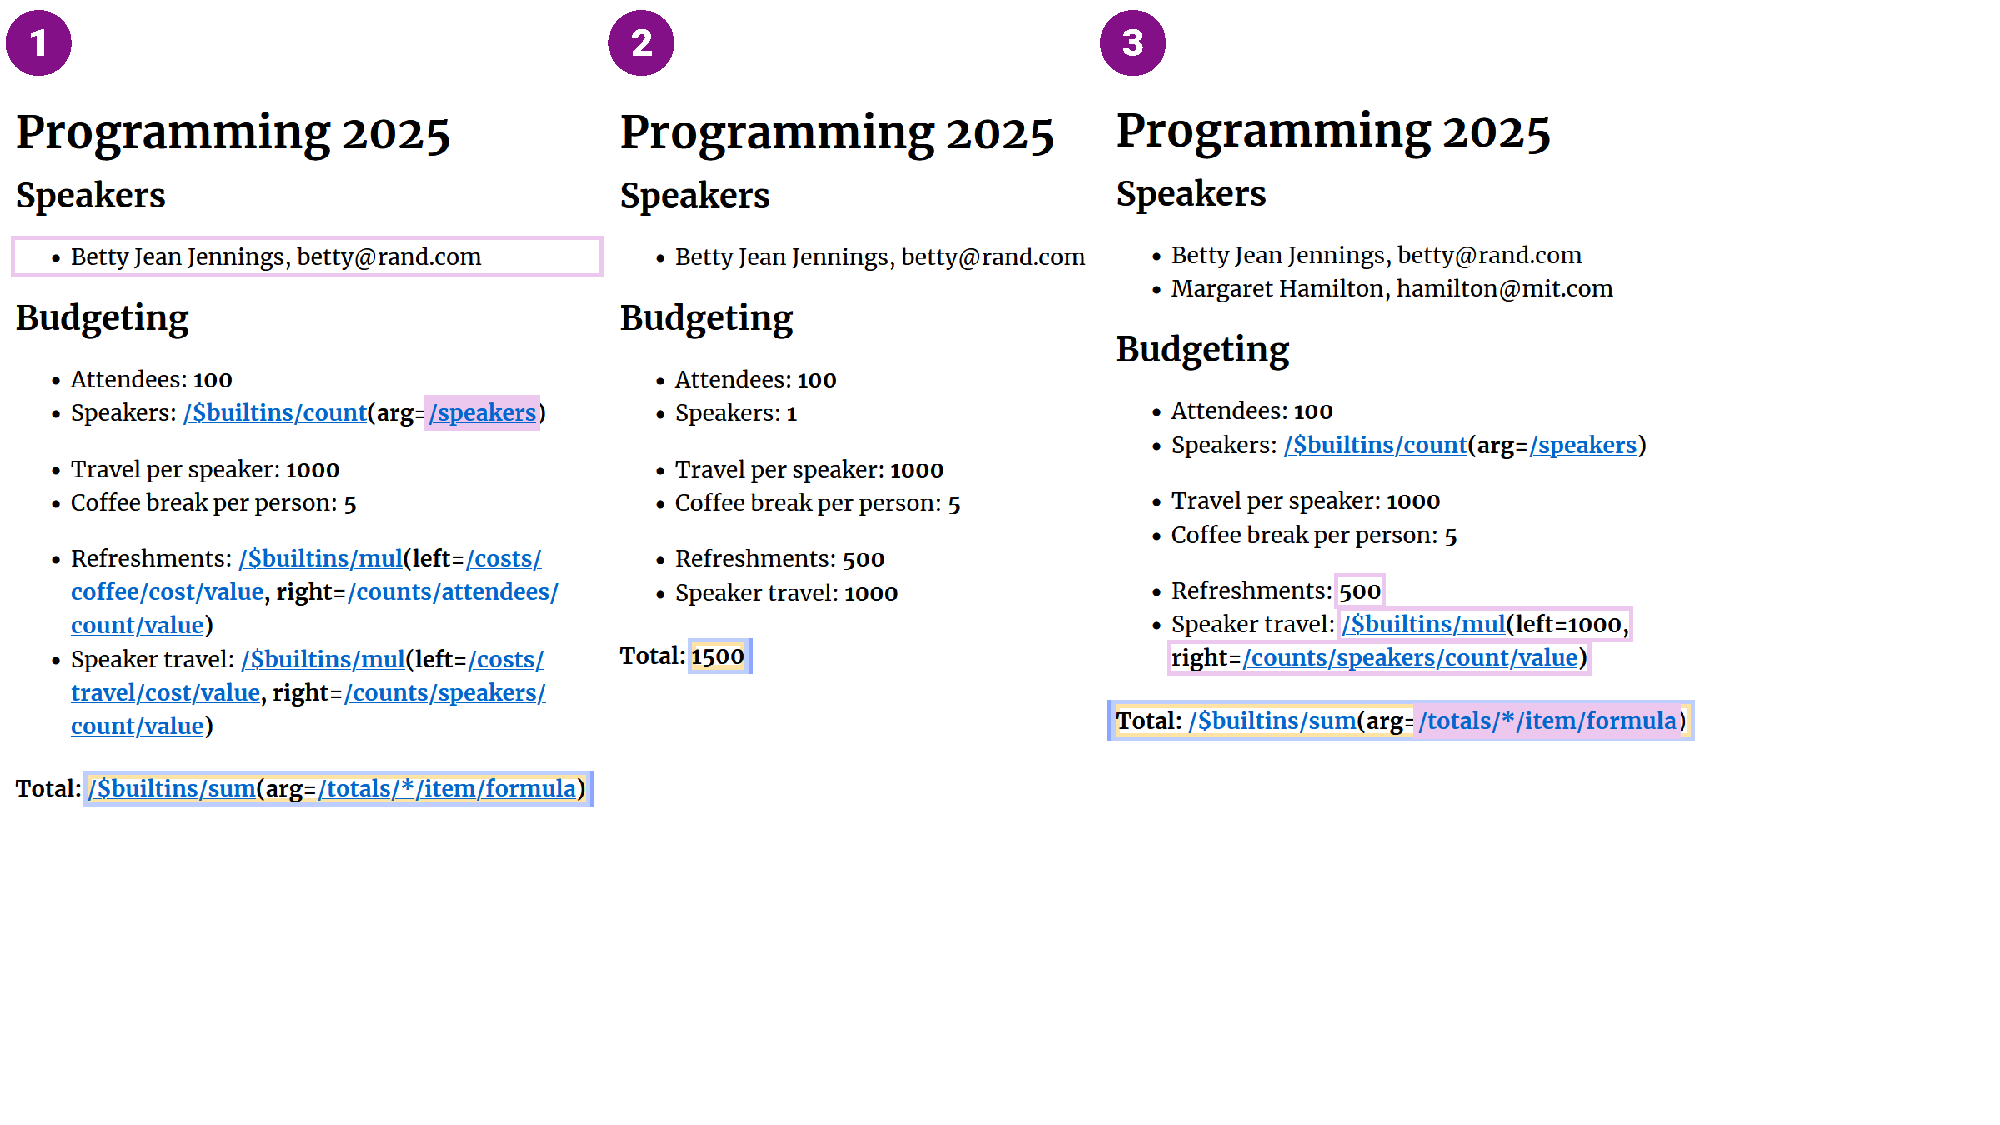
\includegraphics[width=1\columnwidth,clip,trim=0.1cm 5cm 5.1cm 0cm]{fig/incremental.pdf}
  \vspace{-1em}
  \caption{Budget calculation based on the number of speakers (1) and the result (2). When speaker
  is added (3), only the results of affected formulas are invalidated.}
  \label{fig:incremental}
  \vspace{-0.5em}
\end{figure}

\newpage

\subsection{Schema code co-evolution}
\label{sec:impl-schema}

\subsection{Provenance tracking}
\label{sec:impl-provenance}

\subsection{Managed copy \& paste}
\label{sec:impl-copy}

% TODO: Start Implementation section with some overall description of the "formative prototype"
% TODO: In operations - better conflict resolution in terms of effect analysis
% (collect selectors with structure/data effects; merging structure x data effects is OK,
% but data x data or structure x structure is not); - Implement this
% TODO: Add a section after Local-First Editing on the new conflict resolution (with demos)
% TODO: In implementation use effects to better replay saved edits
% (push through new structural but not data edits)

\section{Design Discussion}
\label{sec:discuss}

save graph of edits rather than list
(would make replaying of saved edits easier because the histhash never changes)

Although Denicek does not explicitly track document structure (or schema, or type), all documents
have an implicit structure.

c.f. notes

memory mapped graphics etc.

unifying lists and records?

AppendFrom - hard to avoid! because recorded edits cannot know length
(but having -1 in index would break too)

\section{Case study}
\label{sec:case}
(data science environment)

\section{Discussion}
\subsection{Heuristic evaluation}
\subsection{Limitations}
\subsection{Future work}
\label{sec:discuss-future}
use type system to check temporarily invalid state

ohter formal things
* non-conditionality of edits
* show that they can transform document from any to any without removing/readding values


PROPERTIES
- can change any document to any other - sure, via remove add - but also more semantically
(if it contained all values, can we do it without removing and adding them?)

maybe



xx
\newpage
xx

~\\
introduction \\
background \\
related work \\
design process / goals \\
case study \\
formative research \\
formative study \\
analysis \\
system \\
implementation \\
evaluation / heuristic evaluation \\
discussion and limitations \\

\newpage

\section{Introduction}

The computational substrate using which software is built determines the capabilities that the
software can provide. An imperative substrate that views programs as instructions modifying
bytes in memory makes it almost impossible to allow end-user inspection or reprogramming of
running software.

A computational substrate defines what software is built from. This may be objects as in
Smalltalk, lists as in Lisp, or memory with data and code as in UNIX/C.
The different substrates enable different kinds of programming experiences.
For example, object-oriented programming has historically been linked to the development
of graphical user interfaces (where objects can correspond to elements on the screen).
It has also enabled the development of visual programming environments such as the Alternate
Reality Kit, based on message sending between objects.

In principle, any computational substrate can be used to develop any programming experience,
but the greater the impedance mismatch between the substrate and the desired experience,
the more difficult it will be to provide the experience and combine it with the rest of the
system and other programming experiences developed for the system. (One can implement support
for programming-by-demonstration using C/C++, for example as part of a game scripting engine,
but it will not work with the rest of the ordinary C/C++ ecosystem.)

\subsection{Substrate}

The question asked in this paper is, what would be the ideal programming substrate
for supporting a range of programming experiences that make programs more
collaborative, transparent and allows for a gradual transition from non-programmer
to a programmer. We want a programming substrate that makes it easy to develop
programming experiences such as:

\begin{itemize}
\item \emph{Programming by demonstration} --
  Allow non-programmers to construct simple programs by performing examples of the expected behaviour. \cite{leiva-2021-rapido}.
\item \emph{Local-first collaboration} --
  Multiple users should be able to use and modify a single program, preferrably without requiring a central server. \cite{kleppmann-2019-local}
\item \emph{Provenance tracking} --
  The execution of the program should leave an understandable trace that lets the user understand why program resulted in a particular result.
\item \emph{Schema evolution [extra-ish]} --
  When the user evolves the structure of the program, data and code should co-evolve automatically to match the new structure.
\item \emph{Notational freedom [extra-ish?]} --
  Allow users to adapt the program using a notation that suits them and is appropriate for the programming task at hand. [Joel]
\item \emph{Concrete programming [extra?]} --
  It should be possible to reuse parts of program or program logic without constructing abstractions, for example by managed copy \& paste.\cite{edwards-2006-copypaste,edwards-2022-copypaste}
\end{itemize}

substrate as defined by \cite{jakubovic-2022-ladder}

% pbd
\cite{leiva-2021-rapido,cypher-1993-pbd}
\cite{chen-2023-miwa}

% lcoal first
\cite{kleppmann-2019-local,klokmose-2024-mywebstrates}
% provenance
\cite{ko-2004-whyline,ko-2009-whyline,krebs-2023-probelog}
\cite{ricciotti-2017-imperative,perera-2012-functional}
\cite{perera-2022-linked}


% visualizations of results or execution
% https://www.dcs.warwick.ac.uk/pvw04/p01.pdf
% https://dl.acm.org/doi/10.1145/3313831.3376494

% previews - livelits

% Schema evolution
% our paper; see https://openproceedings.org/2023/conf/edbt/paper-160.pdf - good refs in 2.2

% https://x.com/jonathoda/status/1185888711210389504

% also cool: https://arxiv.org/pdf/2303.06777

% Hazel family of things
% structure editing - sandblocks

Joel's definition of substrate in Onward!
Bret Victor talk
\url{https://www.youtube.com/watch?v=ef2jpjTEB5U}

In what ways is a substrate "natural"?

thinglab - create line by cloning, it sticks to mouse pointer, clicking sticks it to something else
squeak - has all the browsers (method search...)


computational substrate
how it differs from computational media?
more low-level - media suggests that there it comes

\section{The whatever system}
\subsection{Document + Edits}
defines
\begin{itemize}
  \item selectors
  \item nodes
  \item edits
\end{itemize}

\subsection{Walkthrough}
* todo list? (or counter, but that is a bit boring)

\section{Themes}
* programming by demonstration
  - binding interactions to gui elements (event handlers)
* provenance tracking
  - Amy Ko's whyline, Probe Log by HPI, enables linked visualizations
* merging of edit histories / collaborative editing
  - bonus - can share restricted link to allow users fill out
    forms (allow partial edits only / def by selector?)
* scehma change - change data \& code accordingly
* everything is an edit
  - interaction with the GUI
  - evaluation? tbd
* copy \& paste abstraction
    (requires finishing new approach to formulas!)
  - edit before copy to propagate edit to other places
    (or edit after copy to make it specific to a case)
  - higher order copying from https://tomasp.net/academic/papers/copy-paste/paint22.pdf
* augmenters
  - cf. bonnie nardi (calls them something else - Jonathan says)
  - add programming by demonstration data wrangling gui to table (trigger interactions)
    cf. lorgnette

\section{Applications}
* todo list / counter / maybe too simple
* (if used in the walkthrough, maybe something else? board game as in varv - tic tac toe? or 7guis?)
* conference organizer
* data exploration (ala histogram)
* linked charts

\section{Extras}
* metablocks?
* self-sustainability
* some non-browser implementation of this (as in Varv?)

explicit structure
self-sustainability
notational freedom

\newpage
~

Maybe have 'enabled' for edits afterall?
(we can merge with conflicts and disable some edits, but keep them in history for info)

NOTES
type Edit =
  { Kind : EditKind
    Dependencies : Selectors list }  -- only needed for evaluated edits

VALUE vs STRUCTURE distinction
* good in theory, nice for implementation
* tricky to use! needs some assistance tools

TODO - things to work on
* "represent" edits somewhere in document as "library of functions"
  and then call those from buttons (rather than embedding them directly)
  allow some kind of abstraction (as in Histogram) to make them reusable
* figure out how to do evaluation better
  (based on the stored abstractions? but need to store provenance...)

SEMANTIC CONDITIONS
\url{https://www.youtube.com/watch?v=NBnc2ToS_j0}
(has a section on this in background)

SUBSTRATE DESIGN PROBLEMS
* selectors - all for structure / index for data
  (but it is useful to allow others...)
  (multiselect also bad for checks!)
* groups/conditions/preconditions
  (c.f. email to jonathan)
  tried conditions on edits; trying groups with check edits
* what to do with "disabled edits"? for example when we remove all checked
  (before, this created edit groups with "check" but if the check was false,
  the group was ignored and this messed up merging - because we wouldn't know if the
  edit had any effect or not)

Evaluation
* evaluated edits have to be migrated to the end
  (if there are conflicts, they are dropped)
  Think of this as maintaining a tree:

  e3
  |
  e2   evaluated
  |  /
  e1
  |
  e0

  this has to be serialized as e0 -> e1 -> e2 -> e3 -> evaluated

  evaluated edits do not became part of the main history
  but hang on the side

ISSUES
* if we merge a thing with saved-interactions with something, hashes will change!

NOTES
* ListAppendFrom - we need this, because we cannot encode this.
* for records, we can RecordAdd(sel, fld, ..) @ Copy(sel @ [Field fld], src) but
  this does not work for lists - because we do not know the index!
  (and we cannot look into current document, because it will differ for saved-interactions)


TODO
* many things with <tag> selectors currently do not work
  (e.g. `matches` for highlighting) because if we collect path of a current node,
  we collect indices and get /some/2/another - and cannot tell if this matches
  /some/<li>/another - we'd have to collect more detailed path info!

INTERACTION
* replay stored event handlers against the old version?
  (this way, adding an item to a speakers list gets migrated \& adds a new table row!)
* simlarly!! we need merge in order to apply edits to multiple targets
  (when you remove all items in a list, the indices change)
  (but I guess we should do this against version at the time of saving too....)

[this \& evaluation = the unreasonable effectiveness of merging]

Notes on storing and reusing edits
* references need to be represented as references so that they get updated
  (NO! not if we reply them against old version, which seems better - but there are 2 design choices)
* how to apply them to multiple targets? use Move to update the selectors instead of
  replacing the prefix manually

IDEA: Type check edit groups to ensure they preserve structure but not individual edits eg when adding list item

CONDITIONALS
https://toby.li/files/p311-radensky.pdf


REMAINING IMPLEMENTATION TODOs:

* Some kind of provenance visualization
* Some kind of matchers/transformers mechanism (ideally to add interactive buttons to tables)
* Apply to all (remove completed in TODO)

\newpage
~

\bibliographystyle{plain}
\bibliography{paper}

\end{document}
